\documentclass[custom,plainsections,30pt]{sciposter}

% Define metadata
\newcommand{\pdfauthors}{Chris Fournier}
\newcommand{\pdftitle}{An Example LaTeX poster}
\newcommand{\pdfemail}{cfour037@eecs.uottawa.ca}
\newcommand{\pdfinstitute}{School of Electrical Engineering and Computer Science\\
University of Ottawa}

% Include packages
\usepackage[pdftex]{graphicx}
\usepackage{tabulary}	% Fancy table column types
\usepackage{amsmath}	% More math 
\usepackage{amsfonts}	% Math fonts
\usepackage{mathtools}	% Math display tools
\usepackage{cases}		% Cases in math
\usepackage{glossaries} % Adds glossaries support; required for some captioning
\usepackage{multirow}	% Multiple table rows
\usepackage{multicol}	% Multiple table columns
\usepackage{comment}	% Comment out sections
\usepackage{color}		% Add colour support
\usepackage[table, x11names, rgb]{xcolor} % Add table colour support, colour names, and rgb specification of colours
\usepackage{soul}		% Highlighting support
\usepackage[normalem]{ulem}	% Underlining support
\usepackage{natbib}		% Better citation styles
\usepackage{caption}
\usepackage{tikz}		% Diagram and drawing library
\usepackage{tikz-qtree}	% Draw trees
\usepackage{pgfplots}	% Charts, requires tikz first
\usepackage{sectsty}	% Set font styles to headings
% Add a variety of tikz packages for drawing
\usetikzlibrary{arrows,automata,shapes}

% Set headings to arial
\allsectionsfont{\usefont{OT1}{phv}{b}{n}\selectfont\centering}

% Set PDF metadata
\usepackage[pdfauthor={\pdfauthors},%
pdftitle={\pdftitle},%
pagebackref=false,%
pdfborder=0 0 0,
pdftex]{hyperref}

% Colour hyperlinks black so that they appear to be normal text
\hypersetup{ 
colorlinks,% 
citecolor=black,%
filecolor=black,% 
linkcolor=black,% 
urlcolor=black
}

% Remove ruler between columns in multicol
\setlength{\columnseprule}{0pt}


% Include the title page setup
\title{\usefont{OT1}{phv}{b}{n}\selectfont \pdftitle}
\author{\pdfauthors}
\institute{\pdfinstitute}
\email{\pdfemail}

% To add, or remove, a left logo
%\noleftlogo
\leftlogo[1]{src/images/UOlogoBW}

% To add, or remove, a right logo (uncommenting \norightlogo can unbalacne the top when only a left logo is present)
%\norightlogo
%\rightlogo[1]{src/images/UOlogoBW}

% For no logos at all
%\nologos

% Create a 3 column poster
\begin{document}
\maketitle
\begin{multicols*}{3} % Use a 3 column poster format

% Set the paragraph indent
\setlength{\parindent}{2em}

% Include various section files

\section*{Introduction}
A poster works just like a regular \LaTeX{} document.  You can create a section
hierarchy using:
\begin{itemize}
  \setlength{\itemindent}{1em}
  \item \verb+\section*{Introduction}+
  \item \verb+\subsection*{A subsection}+
  \item \verb+\subsubsection*{A sub sub section}+
  \item \verb+\paragraph*{A bolded text label for a paragraph}+
\end{itemize}

\noindent To customize various elements such as the:
\begin{description}
  \setlength{\itemindent}{1em}
  \item[Poster size], edit the \verb+papercustom.cfg+ file;
  \item[Title, authors, etc.], edit the top of the \verb+paper.tex+ file;
  \item[Title format], edit the \verb+title.tex+ file.
\end{description}

\noindent For more information on \LaTeX, view the the WikiBook \citet{wikibook:latex} as a reference.
If you are having trouble with something in \LaTeX, ask a question on \url{http://tex.stackexchange.com/}.

For this poster, a slight modification of the \verb+sciposter+ \citep{website:sciposter} package is used.
Refer to the \verb+sciposter+ manual \citep{manual:sciposter} for more detailed information on the package and the various options it offers.

\section*{Motivation}
You should ideally provide some motivation for your work.
The motivation for this work is the creation of interesting charts and graphs!


\section*{Examples of Various Packages}

\subsection*{TiKZ and PGF}
TiKZ and PGF \citep{website:pgf} allow you to create graphics within \LaTeX.
There are plenty of examples of various figures at \url{http://www.texample.net/tikz/}.
Refer to the PGF \citep{manual:tikz_pgf} manual for a reference and tutorial.


% Definition of circles
\def\firstcircle{(0,0) circle (1.5cm)}
\def\secondcircle{(0:2cm) circle (1.5cm)}

\colorlet{circle edge}{blue!50}
\colorlet{circle area}{blue!20}

\tikzset{filled/.style={fill=circle area, draw=circle edge, thick},
    outline/.style={draw=circle edge, thick}}


\begin{table}
\centering
\begin{tabular}{ c c }
% Set A and B
\begin{tikzpicture}[scale=2]
    \begin{scope}
        \clip \firstcircle;
        \fill[filled] \secondcircle;
    \end{scope}
    \draw[outline] \firstcircle node {$A$};
    \draw[outline] \secondcircle node {$B$};
    \node[anchor=south] at (current bounding box.north) {$A \cap B$};
\end{tikzpicture}
&
%Set A or B but not (A and B) also known a A xor B
\begin{tikzpicture}[scale=2]
    \draw[filled, even odd rule] \firstcircle node {$A$}
                                 \secondcircle node{$B$};
    \node[anchor=south] at (current bounding box.north) {$\overline{A \cap B}$};
\end{tikzpicture}
\\
% Set A or B
\begin{tikzpicture}[scale=2]
    \draw[filled] \firstcircle node {$A$}
                  \secondcircle node {$B$};
    \node[anchor=south] at (current bounding box.north) {$A \cup B$};
\end{tikzpicture}
&
% Set A but not B
\begin{tikzpicture}[scale=2]
    \begin{scope}
        \clip \firstcircle;
        \draw[filled, even odd rule] \firstcircle node {$A$}
                                     \secondcircle;
    \end{scope}
    \draw[outline] \firstcircle
                   \secondcircle node {$B$};
    \node[anchor=south] at (current bounding box.north) {$A - B$};
\end{tikzpicture}
\\
% Set B but not A
\begin{tikzpicture}[scale=2]
    \begin{scope}
        \clip \secondcircle;
        \draw[filled, even odd rule] \firstcircle
                                     \secondcircle node {$B$};
    \end{scope}
    \draw[outline] \firstcircle node {$A$}
                   \secondcircle;
    \node[anchor=south] at (current bounding box.north) {$B - A$};
\end{tikzpicture}
& \\
\end{tabular}
\captionof{figure}{TiKZ example of set operations and Venn diagrams by \citet{website:example_venndiag}}
\end{table}


\newcommand{\D}{7} % number of dimensions (config option)
\newcommand{\U}{7} % number of scale units (config option)

\newdimen\R % maximal diagram radius (config option)
\R=3.5cm 
\newdimen\L % radius to put dimension labels (config option)
\L=4cm

\newcommand{\A}{360/\D} % calculated angle between dimension axes  

\begin{centering}
\centering
\hspace{0.5em} % It's centered, but we want the body to be centered, not just the graphic
\begin{tikzpicture}[scale=2]
  \path (0:0cm) coordinate (O); % define coordinate for origin

  % draw the spiderweb
  \foreach \X in {1,...,\D}{
    \draw (\X*\A:0) -- (\X*\A:\R);
  }

  \foreach \Y in {0,...,\U}{
    \foreach \X in {1,...,\D}{
      \path (\X*\A:\Y*\R/\U) coordinate (D\X-\Y);
      \fill (D\X-\Y) circle (1pt);
    }
    \draw [opacity=0.3] (0:\Y*\R/\U) \foreach \X in {1,...,\D}{
        -- (\X*\A:\Y*\R/\U)
    } -- cycle;
  }

  % define labels for each dimension axis (names config option)
  \path (1*\A:\L) node (L1) { Security};
  \path (2*\A:\L) node (L2) { Content Quality};
  \path (3*\A:\L) node (L3) { Performance};
  \path (4*\A:\L) node (L4) { Stability};
  \path (5*\A:\L) node (L5) { Usability};
  \path (6*\A:\L) node (L6) { Generality};
  \path (7*\A:\L) node (L7) { Popularity};

  % for each sample case draw a path around the web along concrete values
  % for the individual dimensions. Each node along the path is labeled
  % with an identifier using the following scheme:
  %
  %   D<d>-<v>, dimension <d> a number between 1 and \D (#dimensions) and
  %             value <v> a number between 0 and \U (#scale units)
  %
  % The paths will be drawn half-opaque, so that overlapping parts will be
  % rendered in a composite color.

  % Example Case 1 (red)
  %
  % D1 (Security): 0/7; D2 (Content Quality): 5/7; D3 (Performance): 0/7;
  % D4 (Stability): 6/7; D5 (Usability): 0/7; D6 (Generality): 5/7;
  % D7 (Popularity): 0/7
  \draw [color=red,line width=1.5pt,opacity=0.5]
    (D1-0) --
    (D2-5) --
    (D3-0) --
    (D4-6) --
    (D5-0) --
    (D6-5) --
    (D7-0) -- cycle;

  % Example Case 2 (green)
  %
  % D1 (Security): 2/7; D2 (Content Quality): 2/7; D3 (Performance): 5/7;
  % D4 (Stability): 1/7; D5 (Usability): 4/7; D6 (Generality): 1/7;
  % D7 (Popularity): 7/7
  \draw [color=green,line width=1.5pt,opacity=0.5]
    (D1-2) --
    (D2-2) --
    (D3-5) --
    (D4-1) --
    (D5-4) --
    (D6-1) --
    (D7-7) -- cycle;

  % Example Case 3 (blue)
  %
  % D1 (Security): 1/7; D2 (Content Quality): 7/7; D3 (Performance): 4/7;
  % D4 (Stability): 4/7; D5 (Usability): 3/7; D6 (Generality): 5/7;
  % D7 (Popularity): 2/7
  \draw [color=blue,line width=1.5pt,opacity=0.5]
    (D1-1) --
    (D2-7) --
    (D3-4) --
    (D4-4) --
    (D5-3) --
    (D6-5) --
    (D7-2) -- cycle;

\end{tikzpicture}
\captionof{figure}{TiKZ example of a spiderweb diagram by \citet{website:example_spiderwebdiagram}}
\end{centering}


\begin{figure}
\centering
\hspace{-4em} % It's centered, but we want the body to be centered, not just the graphic
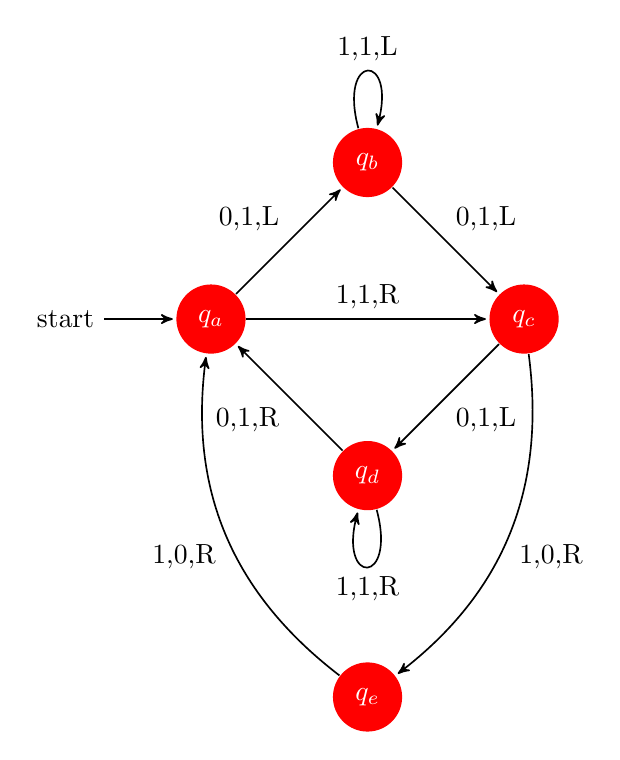
\begin{tikzpicture}[->,>=stealth',shorten >=1pt,auto,node distance=8em,
                    semithick,scale=2]
  \tikzstyle{every state}=[fill=red,draw=none,text=white]

  \node[initial,state] (A)                    {$q_a$};
  \node[state]         (B) [above right of=A] {$q_b$};
  \node[state]         (D) [below right of=A] {$q_d$};
  \node[state]         (C) [below right of=B] {$q_c$};
  \node[state]         (E) [below of=D]       {$q_e$};

  \path (A) edge              node {0,1,L} (B)
            edge              node {1,1,R} (C)
        (B) edge [loop above] node {1,1,L} (B)
            edge              node {0,1,L} (C)
        (C) edge              node {0,1,L} (D)
            edge [bend left]  node {1,0,R} (E)
        (D) edge [loop below] node {1,1,R} (D)
            edge              node {0,1,R} (A)
        (E) edge [bend left]  node {1,0,R} (A);
\end{tikzpicture}
\captionof{figure}{TiKZ example of a state machine by \citet{website:example_statemachine}}
\end{figure}


\subsubsection*{TiKZ-QTree}
TiKZ-QTree is a package specifically designed to make parse trees.
For more information see the manual \citep{manual:tiks_qtree}.

\begin{centering}
\begin{tikzpicture}
\tikzset{level distance=60pt, scale=1.5}
\Tree [.S [.NP [.Det the ] [.N cat ] ]
[.VP [.V sat ]
[.PP [.P on ]
[.NP [.Det the ] [.N mat ] ] ] ] ]
\end{tikzpicture}
\captionof{figure}{Parse tree example from \citet{manual:tiks_qtree}}
\end{centering}



\subsection*{PGF Plots}
The \verb+pgfplots+ package \citep{website:pgfplots} is an extension to allow for easy plotting of charts.

\begin{centering}
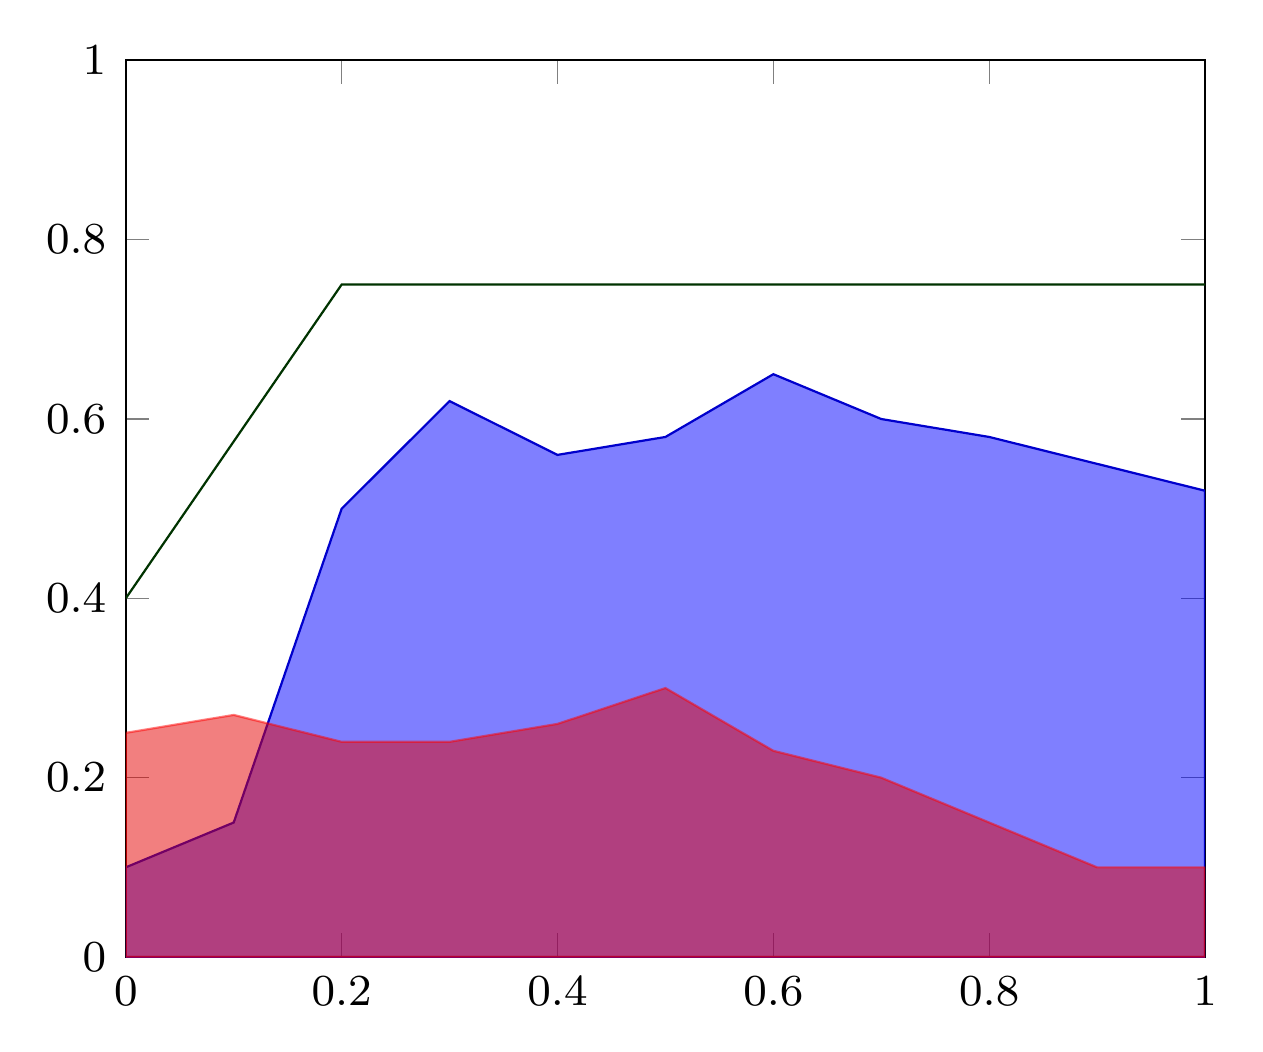
\begin{tikzpicture}[scale=2,font=\footnotesize]
\begin{axis}[ymin=0,ymax=1,enlargelimits=false]
\addplot
    [blue!80!black,fill=blue,fill opacity=0.5]
coordinates
{(0,0.1)    (0.1,0.15)  (0.2,0.5)   (0.3,0.62)
 (0.4,0.56) (0.5,0.58)  (0.6,0.65)  (0.7,0.6)
 (0.8,0.58) (0.9,0.55)  (1,0.52)}
|- (axis cs:0,0) -- cycle;
\addplot
    [red,fill=red!90!black,opacity=0.5]
coordinates
{(0,0.25)   (0.1,0.27)  (0.2,0.24)  (0.3,0.24)
 (0.4,0.26) (0.5,0.3)   (0.6,0.23)  (0.7,0.2)
 (0.8,0.15) (0.9,0.1)   (1,0.1)}
|- (axis cs:0,0) -- cycle;
\addplot[green!20!black] coordinates
    {(0,0.4) (0.2,0.75) (1,0.75)};
\end{axis}
\end{tikzpicture}
\captionof{figure}{Plot example from \citet[p. 21]{manual:pgfplots}}
\end{centering}

\vspace{2em}

\begin{centering}
\begin{tikzpicture}[scale=2,font=\footnotesize]
\begin{axis}
\addplot+[error bars/.cd,y dir=plus,y explicit]
         coordinates {
             (0,0)     +- (0.5,0.1)
             (0.1,0.1) +- (0.05,0.2)
             (0.2,0.2) +- (0,0.05)
             (0.5,0.5) +- (0.1,0.2)
             (1,1)     +- (0.3,0.1)};
\end{axis}
\end{tikzpicture}
\captionof{figure}{Plot example from \citet[p. 205]{manual:pgfplots}}
\end{centering}


\section*{Conclusion}
Hopefully you have been convinced to create a poster using \LaTeX and the various graphical libraries available.

% Setup the bibliography
\begin{small}
\bibliographystyle{agsm} % Harvard = agsm
\bibliography{src/bib/manuals,src/bib/packages,src/bib/examples}
\end{small}

\end{multicols*}
\end{document}
